% !TEX encoding = UTF-8 Unicode
%!TEX root = thesis.tex
% !TEX spellcheck = en-US
%%=========================================
\chapter{Interface between Simulator and Control System}
This chapter will aim to decide an overall layout of the interface between the HIL Simulator and the USV control system to be tested. It will also be suggested an overview of the information flow between important modules of the simulator. Only a general layout will be suggested as the primary simulation target (Odin) is still under development and many details about the HW and SW solutions on board the USV are yet to be decided.

\newpage
\section{Overview of the Simulation Setup}
\begin{wrapfigure}[21]{r}{0.6\textwidth}
	\vspace{-40pt}
	\begin{center}
		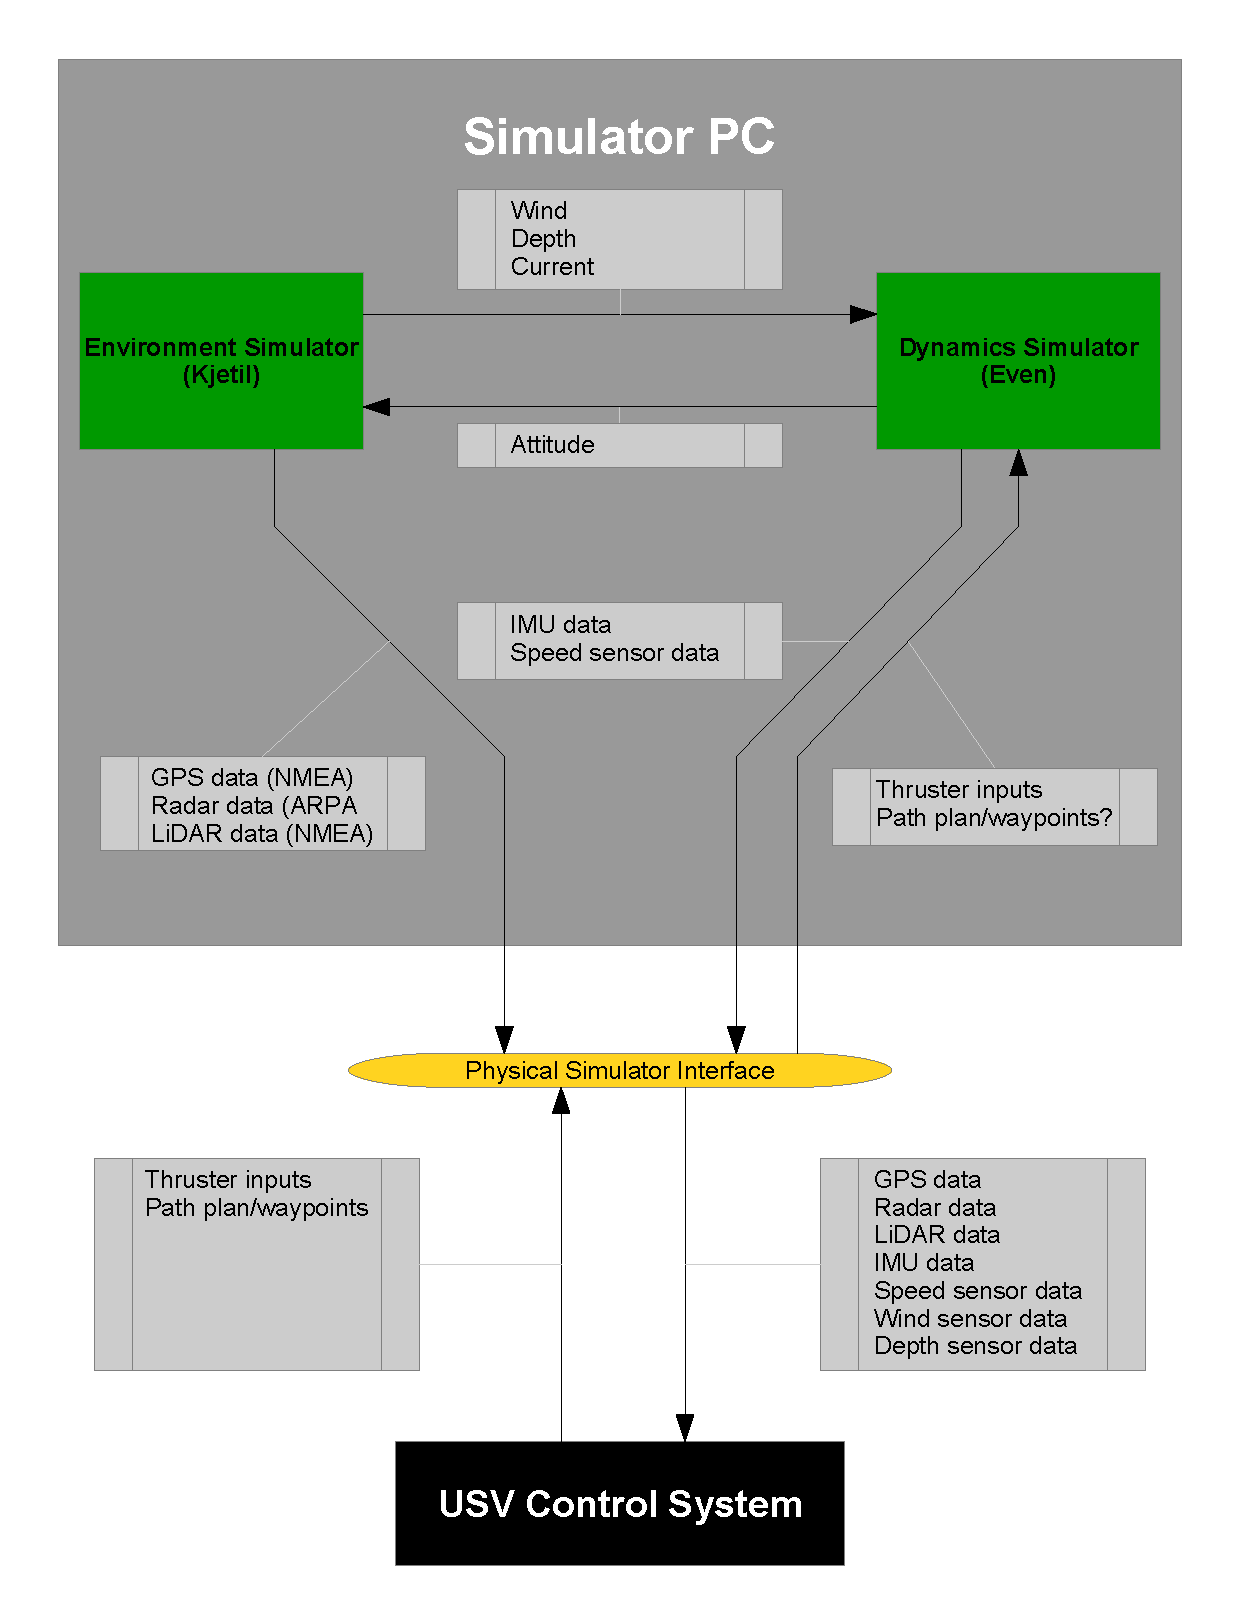
\includegraphics[width= \linewidth]{fig/Interface.pdf}
		\vspace{-40pt}
		\caption{\it{General overview of the planned design of the HIL Simulation setup. The overview includes general information flow between the USV control system, simulator and main software modules.}}
		\label{fig:simLayout}
	\end{center}	
\end{wrapfigure}

The HIL Simulator should be run on a single laptop. The operating system (OS) should be Ubuntu to be able to utilize ROS functionality during simulation. The task of developing the simulator is divided in two projects- and master thesis's: one for the simulation of the surrounding environment around the USV (this project) and one for the simulation of the USV dynamics (\cite{even}). The dividing in two tasks makes it natural to split the simulation software in two main modules: Dynamics and Environment as seen in Figure \ref{fig:simLayout}. The boats attitude and movement at any time are calculated in the Dynamics module. This information should be sent to the Environment module which decides the USV's global position in the simulation environment. Weather conditions such as wind and current are decided in the Environment module and sent to the Dynamics module which calculates how these factors influences the motion of the USV. The two modules, knowing everything about the surroundings and attitude of the USV, generates appropriate sensor data and sends this to the physical interface connecting the HIL Simulator to the USV control system. 

\subsection{Information Flow Between Software Modules}


\section{Physical Interface}
Too early to decide the details of this.

